\documentclass[a4paper,10pt]{article}
\usepackage[utf8x]{inputenc}
\usepackage[italian]{babel}
\usepackage{hyperref}
\usepackage{amsfonts}
\usepackage{graphicx}
\usepackage{amsmath}
\usepackage{subfigure}
\usepackage{placeins}

%opening
\title{Obstacle Avoidance con Potenziali Artificiali per un quadrirotore controllato in Feedback Linearization}
\author{Davide Aversa - Vittorio Perera}

\begin{document}

\maketitle

%\begin{comment}
\begin{abstract}

In questo progetto affronteremo la progettazione e la simulazione di un Quadrirotore UAV dotato di un sistema di navigazione autonomo basato su \emph{Potenziali Artificiali} e controllato in \emph{Feedback Linearization}.

Per prima cosa analizzeremo e simuleremo il controlore con l'ausilio di \emph{MATLAB} e fornendo un modello \emph{Simulink} del sitema.

Nella seconda parte convertiremo il modello in C++ e lo integreremo in \emph{ROS} per fornire una simulazione 3D del quadrirotore all'interno del simulatore \emph{Gazebo}.

Infine, aggiungeremo il modulo di Obstacle Avoidance basato sui Potenziali Artificiali valutandone le performance all'interno dell'ambiente simulato.

\end{abstract}
%\end{comment}

\section{Modello Dinamico}

Nel quadrirotore reale tutti i movimenti sono la conseguenza dalla velocità delle pale, due delle quali ruotano in senso orario (\emph{pale rotanti}) mentre le altre ruotano in senso antiorario (\emph{pale anti-rotanti}). Tali rotazioni generano quattro forze dirette lungo l'asse di rotazione e con modulo proporzionale alla velocità di rotazione

\begin{equation}
F_i = b \Omega_i^2
\end{equation}

dove $b$ è il \emph{coefficente} di thrust delle eliche e $\Omega_i$ è la velocità di rotazione della pala i-esima.

Variando la velocità delle pale è possibile quindi variare il modulo di tali forze e, di conseguenza, impartire al quadrirotore i movimenti desiderati. Ad esempio, generare una differenza di velocità tra le pale poste sullo stesso asse causa la rotazione lungo l'asse opposto inclinando il mezzo (\emph{roll} o \emph{pitch}) con conseguente movimento in direzione della pala a velocità minore. Analogamente, tramite la differenza tra la velocità delle pale rotanti e quelle anti-rotanti è possibile far ruotare il quadrirotore lungo il suo asse verticale (\emph{yaw}).

Dal punto di vista del controllo però risulta più semplice considerare queste quattro forze ascensionali come l'unione di una forza diretta verso l'asse verticale del quadrirotore applicata nel suo centro di massa ($U_1$) e di tre coppie di rotazione lungo \emph{roll}, \emph{pitch} e \emph{yaw} ($U_2$, $U_3$ e $U_4$). La trasformazione in question è data dalle seguenti equazioni:

\begin{equation}
\begin{split}
U_1 &= F_1 + F_2 + F_3 + F_4; \\
U_2 &= F_3 - F_1; \\
U_3 &= F_4 - F_2; \\
U_4 &= F_4+F_2 - F_3 -F_1.
\end{split}
\end{equation}

Il mezzo si comporta allo stesso modo di un corpo rigido nello spazio e le nuove forze $U_1$, $U_2$, $U_3$ e $U_4$ rappresentano gli ingressi del nostro sistema. Questi ingressi possono poi essere riportati indietro alla velocità delle singole eliche tramite la seguente trasformazione inversa:

\begin{equation}
\begin{split}
\Omega_1 &= 2 \sqrt{\frac{U_1 - 2U_2 - U_4}{b}} ; \\
\Omega_2 &= 2 \sqrt{\frac{U_1 - 2U_3 + U_4}{b}} ; \\
\Omega_3 &= 2 \sqrt{\frac{U_1 + 2U_2 - U_4}{b}} ; \\
\Omega_4 &= 2 \sqrt{\frac{U_1 + 2U_3 + U_4}{b}}.
\end{split}
\end{equation}

A questo punto, senza entrare in dettaglio\footnote{La derivazione del modello totale è trattata in dettaglio nella relazione di Giovanni Mattei e Riccardo Sven Risuleo}, possiamo esprimere il modello totale del quadrirotore come:

\begin{equation}
\begin{split}
\label{modello_totale}
\dot{x}_0 &= v_x\\
\dot{y}_0 &= v_y\\
\dot{z}_0 &= v_z\\
\dot{\varphi} &= p + \sin \varphi \tan \theta q + \cos \varphi \tan \theta r \\
\dot{\theta} &= \cos\varphi q - \sin \varphi r\\
\dot{\psi} &= \dfrac{\sin \varphi}{\cos \theta} q + \dfrac{\cos \varphi}{\cos \theta} r\\
\dot{v}_x &= - \dfrac{1}{2m}\rho_{air}C_x v_x\sqrt{v_x^2+v_y^2+v_z^2} + \dfrac{1}{m}\left(\sin\varphi \sin\psi + \cos\varphi \cos\psi \sin\theta\right)U_1\\
\dot{v}_y &= - \dfrac{1}{2m}\rho_{air}C_y v_y\sqrt{v_x^2+v_y^2+v_z^2}  + \dfrac{1}{m}\left(\cos\varphi \sin\psi \sin\theta - \cos\psi \sin\varphi\right)U_1\\
\dot{v}_z &= - \dfrac{1}{2m}\rho_{air}C_z v_z\sqrt{v_x^2+v_y^2+v_z^2}  - g + \dfrac{1}{m} \cos\varphi \cos\theta U_1 \\
\dot{p} &= \dfrac{I_y -I_z}{I_x}qr - \dfrac{1}{2I_x}\rho_{air}C_pp\sqrt{p^2+q^2+r^2} + \dfrac{I_r}{I_x} q \Omega_m +  \dfrac{l}{I_x}U_2\\
\dot{q} &= \dfrac{I_z -I_x}{I_y}pr - \dfrac{1}{2I_y}\rho_{air}C_qq\sqrt{p^2+q^2+r^2}  - \dfrac{I_r}{I_y} p \Omega_m +  \dfrac{l}{I_y}U_3\\
\dot{r} &= \dfrac{I_x -I_y}{I_z}pq - \dfrac{1}{2I_z}\rho_{air}C_rr\sqrt{p^2+q^2+r^2}  + \dfrac{d}{I_z}U_4\\
\end{split}
\end{equation}

Dove abbiamo le seguenti variabili di stato

\begin{enumerate}
\item $x_0$, $y_0$ e $z_0$ rappresentano la posizione del centro di massa del quadrirotore.
\item $\varphi$, $\theta$ e $\psi$ rappresentano l'orientamento del quadrirotore nella terna RPY.
\item $v_x$, $v_y$ e $v_z$ rappresentano la velocità lineare del centro di massa del quadrirotore.
\item $p$, $q$ e $r$ è una terna che rappresenta la velocità angolare del quadrirotore.
\end{enumerate}

e le seguenti costanti

\begin{enumerate}
\item $m$ è la massa del quadrirotore.
\item $\rho_{air}$ è il \emph{coefficiente di densità dell'aria}.
\item $C_x$, $C_y$, $C_z$, $C_p$, $C_q$ e $C_r$ sono coefficenti aerodinamici dipendenti dalla forma del quadrirotore e che modellano la resistenza dell'aria che subisce il quadrirotore muovendosi rispettivamente lungo $x$, $y$ e $z$ e con velocità angolare $p$, $q$ e $r$.
\item $I_x$, $I_y$ e $I_z$ sono i coefficienti di inerzia del quadrirotore.
\item $l$ rappresenta la lunghezza delle braccia del quadrirotore.
\item $d$ è il \emph{coefficente di drag} delle eliche.
\item $g$ è semplicemente l'accelerazione gravitazionale terrestre.
\end{enumerate}

A questo punto abbiamo tutto quello che ci serve per poter progettare il nostro controllore.

\subsubsection*{Riferimenti Bibliografici}

Teoria sulla modellizzazione del quadrirotore [\cite{Mistler2001}]
\newpage
\section{Feedback Linearization}

\subsection{Analisi}

La \emph{feedback linearization} è un comune approccio per il controllo di \emph{sistemi non-lineari} come, ad esempio, quello del quadrirotore. Dato un sistema del tipo

\begin{equation}
\begin{split}
\dot{x} &= f(x) + g(x)u \qquad x \in \mathbb{R}^{n}\, y \in \mathbb{R}^{m} \, u \in \mathbb{R}^{p}; \\
y &= h(x).
\label{eq:nonlinear}
\end{split}
\end{equation}

lo scopo della feedback linearization è di trovare un ingresso

\begin{equation}
u = \alpha(x) + \beta(x)v
\label{eq:u}
\end{equation}

tale che il sistema (\ref{eq:nonlinear}) si comporti come un sistema lineare completamente raggiungibile del tipo

\begin{equation}
\begin{split}
\dot{z} &= Az + Bv; \\
y &= Cx.
\end{split}
\label{eq: linear}
\end{equation}

dove $v$ rappresenta il nuovo ingresso del sistema linearizzato e $z$ rappresenta una nuovo stato ottenuto tramite $\Phi(x)$ \footnote{In particolare $\Phi$ deve essere un \emph{diffeomorfismo globale} ovvero una funzione invertibile di classe $\mathcal{C}^{\infty}$ in cui anche la sua inversa è di classe $\mathcal{C}^{\infty}$.} una trasformazione di variabili completamente invertibile .

Per applicare la feedback linearization al nostro quadrirotore, per prima cosa, è necessario scegliere un sottoinsieme delle variabili di stato che definiscono il nostro \emph{obiettivo di controllo}. Per evitare complicazioni, scegliamo un numero di uscite pari al numero di ingressi in modo da avere un sistema perfettamente controllabile. Nel caso del quadrirotore quindi sceglieremo di controllare la posizione $(x,y,z)$ e l'angolo di $yaw$.

\begin{equation}
y = [x,y,z,\psi]^T
\end{equation}

A questo punto consideriamo il vettore $(r_1,r_2,r_3,r_4)$ contenente il \emph{grado relativo del sistema per ogni uscita}. Tale valore indica il numero di volte che bisogna differenziare $y_i$ per ottenere una dipendenza diretta dall'ingresso $u$.

Differenziando ogni elemento del vettore di uscita per il proprio grado relativo otteniamo

\begin{equation}
\left[ \begin{array}{c} y^{(r_1)} \\ y^{(r_2)} \\ y^{(r_3)} \\ y^{(r_4)} \end{array} \right] = l(x) + J(x)u
\label{eq:lju}
\end{equation}

dove

\begin{equation}
J(x) = \begin{bmatrix} L_{g_1}(L^{{r}_{\scriptsize{1}}-1}_f(h_1)) & \cdots & L_{g_m}(L^{{r}_{\scriptsize{1}}-1}_f(h_1))\\ \vdots & \vdots & \vdots \\ L_{g_1}(L^{{r}_{\scriptsize{m}}-1}_f(h_m)) & \cdots & L_{g_m}(L^{{r}_{\scriptsize{m}}-1}_f(h_m)) \end{bmatrix}
\end{equation}

e 

\begin{equation}
l({x}) = \begin{bmatrix} L^{{r}_{\scriptsize{1}}}_f(h_1)\\ \vdots \\ L^{{r}_{{\scriptsize{m}}}}_f(h_m) \end{bmatrix}
\end{equation}

Invertendo la (\ref{eq:lju}) otteniamo

\begin{equation}
\begin{split}
\alpha(x) &= -J^{-1}(x)l(x); \\
\beta(x) &= J^{-1}(x).
\end{split}
\end{equation}

e, inserendo tutto in (\ref{eq:u}) 

\begin{equation}
u = J^{-1}(x)[ -l(x) + v]
\label{eq:control_input}
\end{equation}

È da notare che questa soluzione è ammissibile se e solo se $J(x)$ è invertibile\footnote{Da notare che il fatto di aver scelto un numero di stati controllabili uguale al numero degli ingressi rende $J(x)$ una matrice quadrata permettendoci di ignorare i problemi aggiuntivi che deriverebbero dall'uso di una pseudo-inversione.}. 

Sfortunatamente nel quadrirotore il vettore dei gradi relativi è $(2,2,2,2)$ e la matrice $J(x)$ è della forma

\begin{equation}
J(x) = \left[ 
\begin{matrix}
J_{1,1} & 0 & 0 & 0 \\ 
J_{2,1} & 0 & 0 & 0 \\ 
J_{3,1} & 0 & 0 & 0 \\ 
0 & 0 & J_{4,3} & J_{4,4}
\end{matrix}
\right]
\end{equation}

Come si può facilmente intuire tale matrice \emph{non} è invertibile per nessun valore di $x$. Per evitare che la matrice sia sempre singolare possiamo ritardare la comparsa di $u_1$ nelle componenti $y^{(2)}_1$, $y^{(2)}_2$ e $y^{(2)}_3$ applicando un \emph{estensione dinamica} al sistema.

Aggiungiamo quindi alle 12 variabili di stato due variabili fittizie 

\begin{equation}
\begin{split}
\dot{U_1} &= \eta \\
\dot{\eta} &= \tilde{U_1}
\end{split}
\end{equation}

ottenendo in questo modo un nuovo sistema nella forma:

\begin{equation}
\dot{\tilde{x}}=\tilde{f}(\tilde{x})+\tilde{g}(\tilde{x})\tilde{U}
\end{equation}

dove

\begin{equation}\begin{split}
\tilde{f}(\tilde{x}) &= \begin{bmatrix} v_x\\                                              
    v_y\\                                                
    v_z\\                                                 
    p+q\sin\varphi\tan\theta +r\cos\varphi\tan\theta\\        
    q\cos\varphi-r\sin\varphi\\                            
    \frac {q\sin\varphi+ r \cos\varphi}{\cos \theta}\\            
    0 \\
    0 \\
    -g \\                      
    \frac{(Iy-Iz)}{Ix}qr + \frac{Ir}{Ix}q\Omega_m\\                   
    \frac{(Iz-Ix)}{Iy}pr - \frac{Ir}{Iy}p\Omega_m\\                    
    \frac{(Ix-Iy)}{Iz}pq 
    \end{bmatrix}\\
    \tilde{g}(\tilde{x}) &= \begin{bmatrix} 0&0&0&0\\ 0&0&0&0\\ 0&0&0&0\\ 0&0&0&0\\ 0&0&0&0\\ 0&0&0&0\\        \frac{1}{m}(\cos \varphi\sin \theta\cos \psi+\sin \varphi\sin\psi)&0&0&0\\ \frac{1}{m}(\cos \varphi\sin \theta\sin \psi-\sin \varphi\cos \psi)&0&0&0\\ \frac{1}{m}\cos \varphi\cos \theta&0&0&0\\ 0&\frac{l}{I_x}&0&0\\ 0&0&\frac{l}{I_y}&0\\ 0&0&0&\frac{d}{I_z} \end{bmatrix} 
\end{split}\end{equation}

 in cui il vettore di ingresso è formato da $\tilde{U_1}$, $U_2$, $U_3$ e $U_4$.

Nel sistema esteso i gradi relativi di $[x,y,z,\psi]$ sono $[4,4,4,2]$ e la corrispettiva matrice $\tilde{J}(x)$ risualta ora invertibile a patto che $U_1$ sia diverso da zero. La condizione non è restrittiva in quando è sempre verificata nel quadrirotore reale fintanto che le pale sono in movimento.

Al sistema lineare (\ref{eq: linear}) così ottenuto si possono applicare tutti i metodi di controllo dei sistemi lineari tempo-invarianti. In particolare, nel caso di asservimento ad una traiettoria $y(t)$:

\begin{equation}
y_d(t) = \begin{bmatrix} y_{1d}(t)\\ y_{2d}(t)\\ y_{3d}(t)\\ y_{4d}(t) \end{bmatrix}
\end{equation}

\noindent definiamo 4 errori di asservimento:

\begin{equation}
e_i = y_{id} - y_i \qquad i = 1,\ldots, 4
\end{equation}

\noindent e per ciascun uscita un numero di coefficienti del polinomio di Hurwitz, pari al grado relativo:

\begin{equation}
c_0^{i},\ldots ,c_{r_i - 1}^{i} \qquad i = 1,\ldots, 4
\end{equation}

\noindent a questo punto abbiamo tutto ciò che ci serve per definire 4 leggi di controllo $v_i$ che assicurano la convergenza asintotica delle quattro uscite alla traiettoria desiderata:

\begin{equation}\begin{split}\label{pddd}
v_1 &= y_{1d}^{(4)} + \sum_{j = 1}^{4} c_{j-1}^{1} e_1^{(j-1)}\\
v_2 &= y_{2d}^{(4)} + \sum_{j = 1}^{4} c_{j-1}^{2} e_2^{(j-1)}\\
v_3 &= y_{3d}^{(4)} + \sum_{j = 1}^{4} c_{j-1}^{3} e_3^{(j-1)}\\
v_4 &= y_{4d}^{(2)} + \sum_{j = 1}^{2} c_{j-1}^{4} e_4^{(j-1)}
\end{split}
\end{equation}

\subsubsection*{Riferimenti Bibliografici}

Teoria e condizioni di linearizzazione \cite{Isidori1986,NonLinearKhalil,NonLinearIsidoril} e applicazione della stessa al modello del quadrirotore \cite{Mistler2001,Al-Hiddabi2009}

\newpage
\section{Obstacle Avoidance}

\subsection{Analisi}

Il campo potenziale artificiale può essere descritto da una funzione $U$ somma di due campi, uno attrattivo e uno repulsivo.

\begin{equation}
U(\mathbf{p}) = U_{rep}(\mathbf{p}) + U_{att}(\mathbf{p})
\end{equation}

A partire da questo è possibile ricavare una forza $F$ in grado di guidare il robot fino al minimo del campo seguendo il rispettivo \emph{gradiente}.

\begin{equation}
F(\mathbf{p}) = F_{att}(\mathbf{p}) + F_{rep}(\mathbf{p}) = - \nabla U_{rep}(\mathbf{p}) - \nabla U_{att}(\mathbf{p})
\end{equation}

L'espressione del campo attrattivo è semplice e può essere espressa semplicemente come

\begin{equation}
U_{att}(\mathbf{p}) = \frac{1}{2} k_a |\mathbf{p}-\mathbf{p}_{goal}|^2
\label{eq:actractive_field}
\end{equation}

dove $p$ è la configurazione corrente del robot e $\mathbf{p}_{goal}$ è la configurazione desiderata. Dall'equazione \ref{eq:actractive_field} ricaviamo $F_{att}$

\begin{equation}
F_{att}(\mathbf{p}) = - k_a (\mathbf{p} - \mathbf{p}_{goal})
\label{eq:attractive_force}
\end{equation}

Per il campo repulsivo invece useremo la seguente formula

\begin{equation}
U_{rep}(\mathbf{p}) = \begin{cases}
\frac{1}{2} k_r  \left( \frac{1}{\rho} - \frac{1}{\rho_{max}} \right)^2 ,& \mbox{if } \rho \le \rho_{max} \\
0 ,& \mbox{if } \rho > \rho_{max}
\end{cases}
\label{eq:repulsive_field}
\end{equation}

dove $\rho$ è espresso come

\begin{equation}
\rho = \underset{x \in \mathcal{CO}}{\operatorname{argmin}}(d(\mathbf{p},x))
\end{equation}

\noindent ovvero la minima distanza fra la configurazione corrente ed ogni altro punto della frontiera dello spazio $\mathcal{C}$-object. Dall'equazione \ref{eq:repulsive_field} ricaviamo

\begin{equation}
F_{rep}(\mathbf{p}) = 
\begin{cases}
 k_r  \left( \frac{1}{\rho} - \frac{1}{\rho_{max}} \right) \frac{1}{\rho^2} \nabla \rho ,& \mbox{if } \rho \le \rho_{max} \\
 0 ,& \mbox{if } \rho > \rho_{max}
\end{cases}
\label{eq:repulsive_force}
\end{equation}

\noindent che è la nostra espressione per la forza repulsiva.

\begin{figure}
\begin{center}
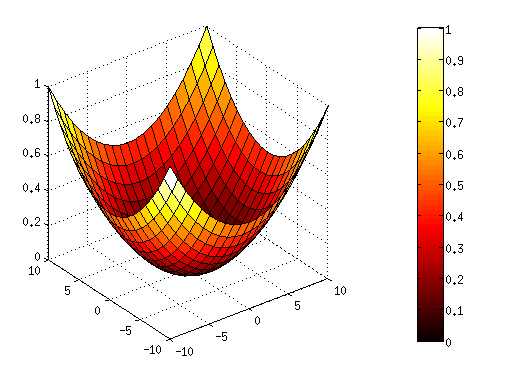
\includegraphics[scale=0.5]{img/attractive.png}
\caption{Un esempio di potenziale attrattivo per uno spazio di configurazione bidimensionale e $\mathbf{p}_{goal} = [0 \, 0]^T$. }
\end{center}
\end{figure}

\begin{figure}
\begin{center}
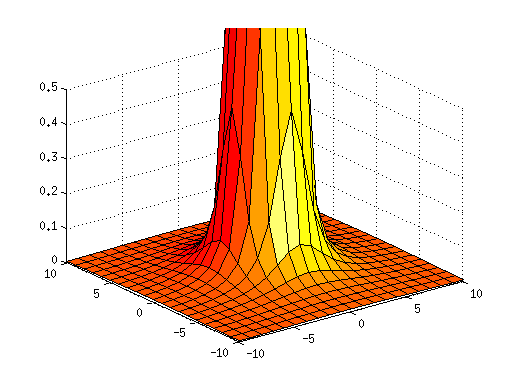
\includegraphics[scale=0.5]{img/repulsive.png}
\caption{Un esempio di potenziale repulsivo per uno spazio di configurazione bidimensionale con un ostacolo circolare di raggio 2 centrato in $\mathbf{p}_{obs} = [0 \, 0]^T$. }
\end{center}
\end{figure}

\subsection{Potenziale artificiale applicato al quadrirotore}

Lo spazio di di configurazione del quadrirotore può essere limitato alle sole variabili controllabili ovvero $x$, $y$, $z$ e lo \emph{yaw} $\psi$. 

\begin{equation}
\mathbf{p} = \left[ 
\begin{matrix}
x \\ y \\ z \\ \psi 
\end{matrix}
\right]
\end{equation}

Costruire la versione in $\mathcal{CO}$ degli ostacoli avvolgiamo il quadrirotore in una sfera di raggio $r$ (Fig. \ref{fig:boundary}) e usiamo la stessa per estendere gli ostacoli reali.

\begin{figure}
\begin{center}
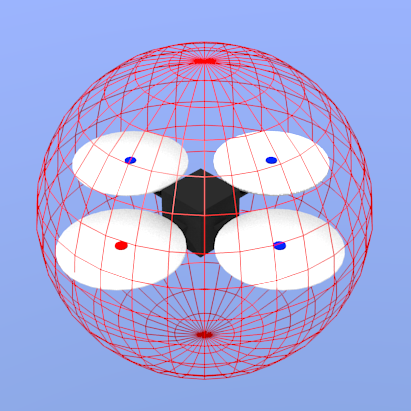
\includegraphics[scale=0.5]{img/boundarysphere.png}
\caption{La sfera (\emph{boundary}) teorica che avvolge il quadrirotore. }
\end{center}
\label{fig:boundary}
\end{figure}

Come conseguenza di questa scelta abbiamo che la distanza minima del quadrirotore da un ostacolo nello spazio delle configurazioni   dipenderà solamente dalla sua distanza dalla posizione $x y z$ del quadrirotore e sarà valida la seguente relazione

\begin{equation}
\rho = \begin{cases}
\rho_{reale} - r ,& \mbox{if } \rho_{reale} \ge r \\
0 ,& \mbox{if } \rho_{reale} < r
\end{cases}
\end{equation} 

\noindent dove $\rho_{reale}$ è la distanza minima del centro di massa del quadrirotore dall'ostacolo più vicino \emph{nello spazio di lavoro}. Tale distanza è immediatamente ricavabile, ad esempio tramite un sensore \emph{laser}.

Un altra conseguenza di questa scelta è che gli ostacoli non influiscono sullo \emph{yaw}. In ogni momento quindi la forza repulsiva sullo \emph{yaw} è nulla

\begin{equation}
F_{rep}(\mathbf{p}) = \left[\begin{matrix}
F_{rep}^x \\
F_{rep}^y \\
F_{rep}^z \\
0
\end{matrix}\right]
\end{equation}

Ora bisogna scegliere come applicare la forza derivante dal campo potenziale artificiale alla feedback linearization del quadrirotore. Partendo dalle 4 leggi di controllo descritte in (\ref{pddd}) possiamo annullare tutti gli errori e imporre

\begin{equation}\begin{split}\label{pot-pddd}
v_1 &= y_{1d}^{(4)} = F_x(\mathbf{p}) + \delta_x \\
v_2 &= y_{2d}^{(4)} = F_y(\mathbf{p}) + \delta_y \\
v_3 &= y_{3d}^{(4)} = F_z(\mathbf{p}) + \delta_z \\
v_4 &= y_{1d}^{(2)} = F_{\psi}(\mathbf{p}) + \delta_{\psi} \\
\end{split}
\end{equation}

Tale assunzione è valida poiché, nel trajectory tracking basato sui potenziali artificiali, assumiamo che il robot si trovi \emph{sempre} sulla traiettoria e, di conseguenza, l'errore è nullo. Il vettore di forze entra nel controllo quindi come \emph{snap} desiderato per quanto riguarda la posizione e come \emph{accelerazione} angolare desiderata dello \emph{yaw}.

Come al solito, quando si imposta un riferimento di ordine superiore al primo, è necessario smorzare il comportamento oscillante o divergente del sistema aggiungendo alla forza un adeguato vettore di \emph{damping} $\mathbf{\delta}$.

\begin{equation}
\mathbf{\delta} = \left[ \begin{matrix}
- k_1 \dot{x} - k_2 \ddot{x} - k_3 \dddot{x} \\ 
- k_1 \dot{y} - k_2 \ddot{y} - k_3 \dddot{y} \\ 
- k_1 \dot{z} - k_2 \ddot{z} - k_3 \dddot{z} \\ 
- k_1 \dot{\psi}
\end{matrix} \right]
\label{eq:damping}
\end{equation}

\subsubsection*{Riferimenti Bibliografici}

Teoria \cite{RoboticsMPC} ed esempi di applicazione \cite{Park2001}.
\newpage

\section{Implementazione}

\subsection{Matlab}

In prima istanza il modello del quadrirotore, il controllore tramite feedback linearization e l'obstacle avoidance tramite artificial potential field sono stati implementati in un modello Simulink.

\subsubsection{Modello del quadrirotore}

\begin{center}
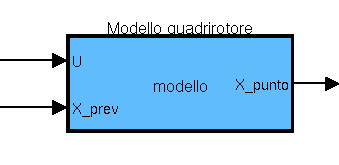
\includegraphics[scale=0.5]{img/quad_model.png} 
\end{center}

Questo primo blocco, ad ogni istante di tempo $t$, prende come input il vettore $U_t$, che rappresenta le variabili di controllo, e lo stato all'istante $t-1$, $x_{t-1}$.  Esso calcola, tramite il modello teorico \ref{modello_totale} del quadrirotore come un corpo rigido a 6 DOF, lo stato $\dot{x}_t$

\subsubsection{Feedback linearization}
\begin{center}
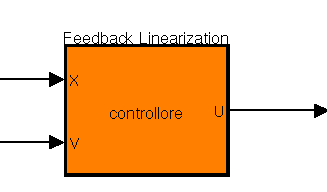
\includegraphics[scale=0.5]{img/feedback.png} 
\end{center}

Questo secondo blocco prende come input lo stato $x$ ottenuto integrando l'uscita del blocco precedente ed il vettore $v$ calcolato in accordo con l'equazione \ref{pddd}. All'interno del blocco vengono calcolate l'inversa della matrice di disaccoppiamento $J$ e il vettore $l$. L'output di questo blocco, ovvero gli input di controllo del sistema, vengono ottenuti applicando la \ref{eq:control_input}.

\subsubsection{Campo Potenziale Artificiale}

\begin{center}
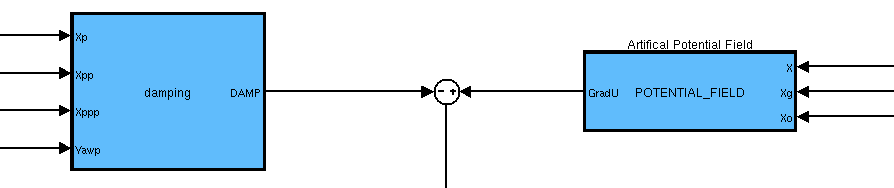
\includegraphics[scale=0.4]{img/potential.png} 
\end{center}

Per calcolare il campo potenziale artificiale abbiamo utilizzato due differenti blocchi. Il primo, sulla destra nell'immagine, prende in input tre vettori $x$, $x_g$ e $x_o$ che rappresentano, rispettivamente, lo stato del quadrotor, la posizione del goal e quella dell'ostacolo. Qesto blocco calcola il valore dei potenziali in accordo con le definizioni delle equazioni \ref{eq:attractive_force} e \ref{eq:repulsive_force}.

Il secondo blocco, sulla sinistra nell'immagine, prende in input lo stato $x$ e le derivate successive fino al terzo ordine. Esso è necessario per introdurre dei fattori di damping $\mathbf{\delta}$ che stabilizzino asintoticamente la convergenza ai valori desiderati in accordo con l'equazione \ref{eq:damping}.

\subsection{GAZEBO e ROS}

Terminato lo sviluppo del modello Simulink, il quadrotor è stato implementato in ROS e GAZEBO.

ROS, acronimo di \emph{Robot Operating system}, ``è un sistema che offre librerie e strumenti atti ad aiutare gli sviluppatori di software a creare applicazioni per robot. In particolare offre un meccanismo di astrazione dell'hardware, drivers, librerie, visualizatori, strumenti per la trasmissione di messaggi, per la gestione dei pacchetti e molto altro''. Nel nostro lavoro ROS è stato utilizzato principalmente come piattaforma per lo scambio di messaggi tra le diverse conponenti del sistema. GAZEBO è invece un simultore multi-robot per ambienti aperti che ci ha permesso di visualizzare i risulatati ma soprattutto di simulare le dinamiche dell'ambiente, del quadrotor e dei sensori.

In fig. \ref{GAZ_ROS} viene rappresentato lo schema a blocchi della simulazione implementata. Il blocco etichettato come GAZEBO simula l'ambiente, il quadrotor ed il sensore laser. Mentre l'ambiente e il quadrotor vengono visualizzati tramite un'interfaccia grafica i dati raccolti dal sensore vengono pubblicati, via ROS, su un apposito topic. Il blocco Feedback Controller, implementato in C++, calcola le forze e le coppie necessarie e le applica al quadrotor nell'ambiente simulato tramite le API di GAZEBO. Le forze e le coppie sono derivate dallo stato attuale del quadrotor, ottenuto direttamente da GAZEBO tramite API, dai rilevamenti del sensore, letti dall'apposito topic di ROS, e dalla posizione del goal. Il goal viene letto da un secondo topic, sempre implementato in ROS, sul quale pubblica il blocco Control Shell; quest'ultimo è una semplice shell implementate in C++ che permette di cambiare dinamicamente il goal del quadrotor.

Nelle simulazioni condotte tramite GAZEBO abbiamo però rilevato che il motore di integrazione su cui si basa crea un grosso rumore numerico. Questo comportamento è ben visibile analizzando l'andamento della velocità angolare dello $\psi$ graficato in fig.\ref{rumore}

\begin{figure}
\begin{center}
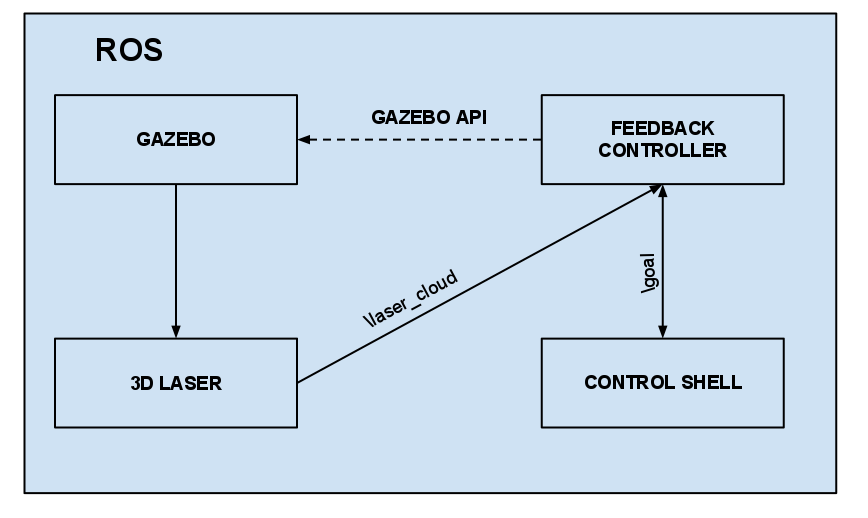
\includegraphics[scale=0.4]{img/gazebo-ros.png}
\end{center}
\caption{Schema a blocchi del modello simulato tramite GAZEBO e ROS}
\label{GAZ_ROS}
\end{figure}


\begin{figure}
\centering
\subfigure[Simulazione complessiva]{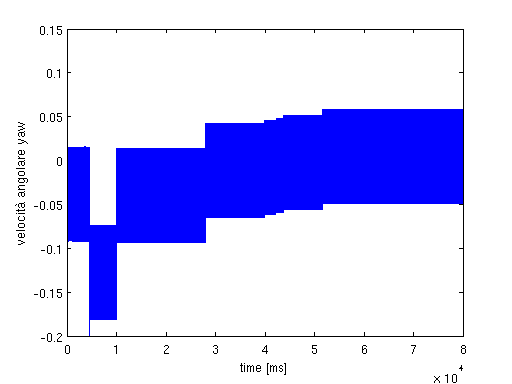
\includegraphics[scale=0.5]{img/plot/gazebo/rumore.png}}
\subfigure[$t=(0,250)$ ms]{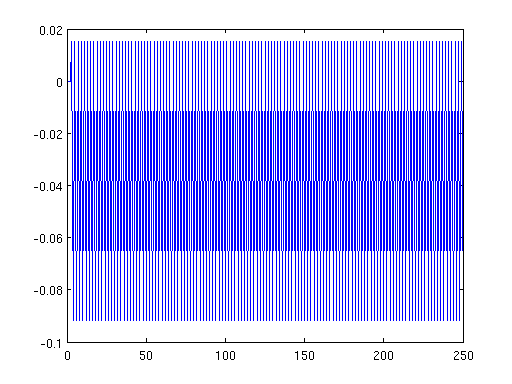
\includegraphics[scale=0.5]{img/plot/gazebo/rumore_zoom.png}}
\caption{Rumore Numerico}
\label{rumore}
\end{figure}
 

\newpage
\FloatBarrier
\section{Simulazioni}
Nelle seguenti simulazione i parametri adottati sono i seguenti:
\begin{center}
\subsubsection*{Guadagni}
\begin{tabular}{|c|c|}
\hline $k_a$ & 3 \\
\hline $k_r$ & 5 \\
\hline $k_y$ & 3 \\
\hline $k_{damping\, vel}$ & 40 \\
\hline $k_{damping\, acc}$ & 20 \\
\hline $k_{damping\, jerk}$ & 10 \\
\hline $k_{damping\, \dot{\psi}}$ & 8\\
\hline
\end{tabular}

\subsubsection*{Parametri Dinamici}
\begin{tabular}{|c|c|}
\hline $mass$ & 0.64 \\
\hline $I_x$ & 0.2 \\
\hline $I_y$ & 0.2 \\
\hline $I_z$ & 0.4 \\
\hline $I_r$ & $10^{-3}$ \\
\hline $g$ & 9.81 \\
\hline $\Omega_m$ & 0\\
\hline $\l$ & 0.165\\
\hline $d$ & $4.5*10^-7$\\
\hline
\end{tabular}


\subsubsection*{Altri Parametri}
\begin{tabular}{|c|c|}
\hline $\rho_{max}$ & 3 \\
\hline $r$ & 0.5 \\
\hline
\end{tabular}
\end{center}

\subsection{Matlab}
\subsubsection*{Simulazione n°1}
In questa prima simulazione lo stato iniziale del quadrotor è $[0,0,7,0]$ mentre il goal è posto in $[7,7,7,-\pi/2]$, è inoltre presente un ostacolo di forma cilindrica e raggio unitario centrato in $[3,5]$.
\begin{figure}
\begin{center}
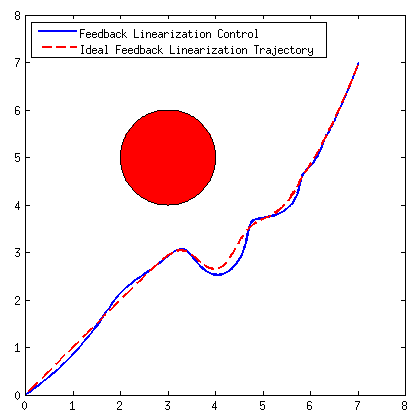
\includegraphics[scale=0.6]{img/plot/matlab/sim1_xy.png}
\end{center}
\caption{Simulazione n°1, Matlab, piano $xy$}
\label{sim:1xy_M}
\end{figure}

In fig. \ref{sim:1xy_M} è rappresentata la traiettoria seguita dal quadrirotrore sul piano $xy$ nell'aggirare l'ostacolo sia nel caso in cui lo stesso sia controllato in \emph{FL} (in blu), sia nel caso di un sistema perfettamente linearizzato simulato con 4 integratori in catena (in rosso). In fig. \ref{sim:1M} vengono invece presentati gli andamenti delle variabili controllate $[ x , y , z , \psi ]$ al variare del tempo.

A prima vista l'andamento è più brusco di quanto si potrebbe immaginare, notiamo infatti una rapida sterzata del quadrirotore in prossimità delle coordinate $<3,3>$. Tuttavia è bene ricordare che le forze repulsive agiscono sul quadrirotore al livello della derivata quarta e che di conseguenza il loro effetto sulla posizione è piuttosto lento. 

Tale comportamento può essere variato e reso più o meno \emph{smooth} giocando con il rapporto fra $k_a$ e $k_r$. Ad esempio, lasciando $k_r$ fisso e diminuendo il guadagno attrattivo si ottiene una traiettoria molto più morbida al prezzo di una minore velocità del mezzo (con $k_a < 3$ il quadrirotore non converge entro i 60 secondi).

\subsubsection*{Simulazione n°2}
In questa seconda simulazione lo stato iniziale ed il goal sono i medesimi della precedente, l'ostacolo però è una sfera centrata in $[4, 4, 8]$. In fig. \ref{sim:2xyz_M} vengono rappresente la traiettorie del quadrotor sui piani $xz$ ed $yz$. Come è facile notare, i due grafici presentano il medesimo andamento come era logico aspettarsi tenendo in considerazione la simmetria del quadrotor e la posizione dell'ostacolo.

Ancora una volta in fig. \ref{sim:2M} vengono presentati gli andamenti delle variabili controllate al variare del tempo.

\begin{figure}
\centering
\subfigure[piano $xz$]{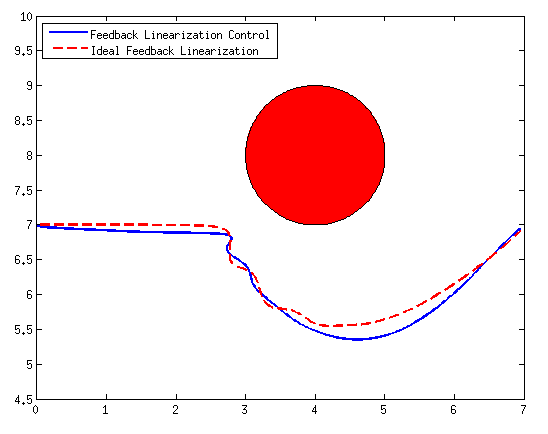
\includegraphics[scale=0.5]{img/plot/matlab/sim2_xz.png}}
\subfigure[piano $yz$]{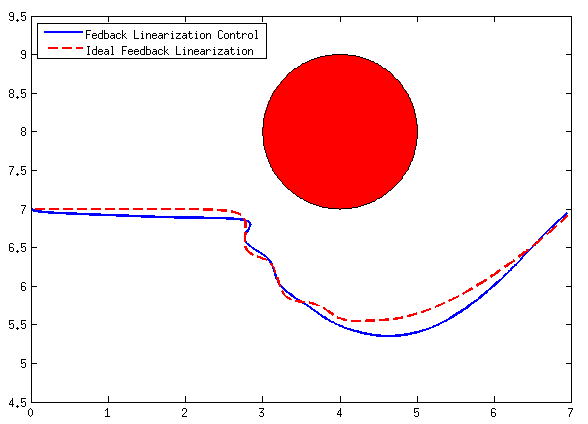
\includegraphics[scale=0.5]{img/plot/matlab/sim2_yz.png}}
\caption{Simulazione n°2, Matlab}
\label{sim:2xyz_M}
\end{figure}


\subsection{GAZEBO}

\subsubsection*{Simulazione n°1}
Le prima simulazione effettuata in GAZEBO riproduce nella maniere più fedele possibile la prima simulazione effettuata in Matlab: stato iniziale e goal sono i medesimi così come i guadagni dei campi attrattivi e repulsivi e il range of influence dell'ostacolo. 
Osservado fig. \ref{sim:1xy_G} possiamo notare che la traiettoria seguita manifesta un andamento oscillante, questo comportamento è da attribuirsi principalmente alla modellazione fisica dell quadrotor che ne "aumenta" le dimensioni e di conseguenza l'ostacolo viene avvertito come più vicino. L'intensità di queste oscillazioni, infatti, dipende sia dal raggio di influenza dell'ostacolo che dal guadagno del campo potenziale repulsivo.

In fig. \ref{sim:1M} vengono riportati gli andamenti delle variabili controllate in funzione del tempo.

\begin{figure}
\centering
\subfigure[piano $xz$]{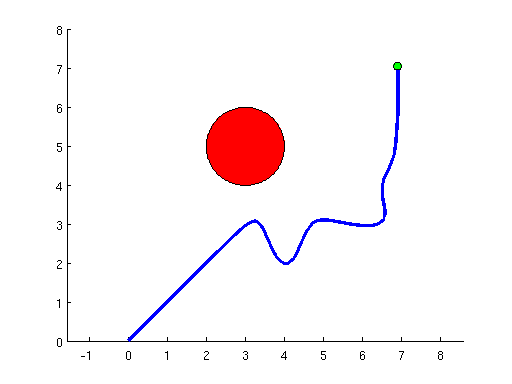
\includegraphics[scale=0.5]{img/plot/gazebo/simulazione1_xy.png}}
\caption{Simulazione n°1, GAZEBO}
\label{sim:1xy_G}
\end{figure}

\subsubsection*{Simulazione n°2}
Anche nella seconda simulazione abbiamo ricalcato la situazione inizialmente presentata su Matlab in GAZEBO, ed anche in questo caso dalla fig. \ref{sim:2xyz_G} osserviamo che la diversa modellazione fisica del quadrotor e gli errori di misurazione introdotti del laser risultano in una traiettoria differente.

In fig. \ref{sim:2G} vengono presentati gli andamenti di tutte e quattro le variabili di controllo al variare del tempo.

\begin{figure}
\centering
\subfigure[piano $xz$]{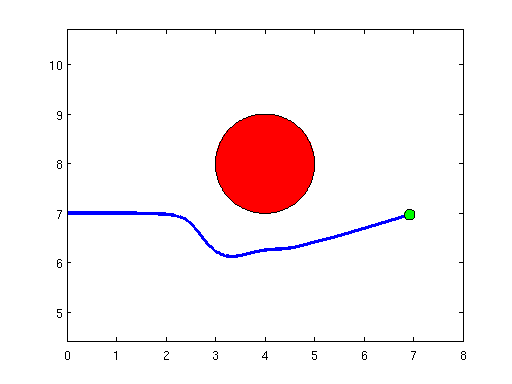
\includegraphics[scale=0.5]{img/plot/gazebo/simulazione2_xz.png}}
\subfigure[piano $yz$]{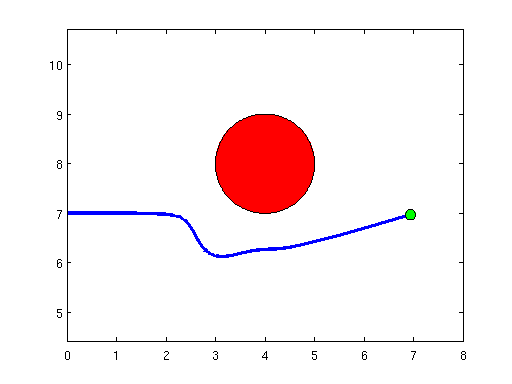
\includegraphics[scale=0.5]{img/plot/gazebo/simulazione2_yz.png}}
\caption{Simulazione n°2, GAZEBO}
\label{sim:2xyz_G}
\end{figure}


\subsubsection*{Simulazione n°3}
In questa terza simulazione lo stato iniziale è $[0,0,7,0]$ ed il goal $[18.5, 17.5, 7, -\pi/2]$. In questo caso sono stati posizionati due ostacoli, di forma cilindrica e raggio unitario, centrati rispetivamente in $[5,3,0]$ e $[13,13,0]$. In fig. \ref{sim:3xy_G} viene rappresentata la traiettoria seguita dal quadrotor sul piano $xy$ ciò che colpisce è il comportamento osservato nell'evitare il secondo ostacolo: una traiettoria che lascia l'ostacolo sulla destra potrebbe sembrare più corretta ma, così facendo, il quadrotor si troverebbe in una posizione più lontana dal goal rispetto a quella raggiunta seguendo la traiettoria tracciata. Scegliere una traiettoria che lascia l'ostacolo sulla destra signifierebbe, di fatto, andare in direzione opposta al gradiente.

Per completezza, in fig. \ref{sim:3G} vengono riportati anche gli andamenti di $[x,y,z,\psi]$ al variare del tempo.

\begin{figure}
\begin{center}
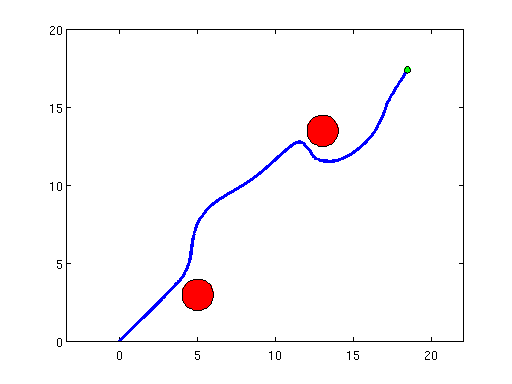
\includegraphics[scale=0.5]{img/plot/gazebo/simulazione3_xy.png}
\end{center}
\caption{Simulazione n°3, GAZEBO, piano $xy$}
\label{sim:3xy_G}
\end{figure}

\newpage
\begin{figure}[p]
\hspace*{-1.5cm}
\begin{center}
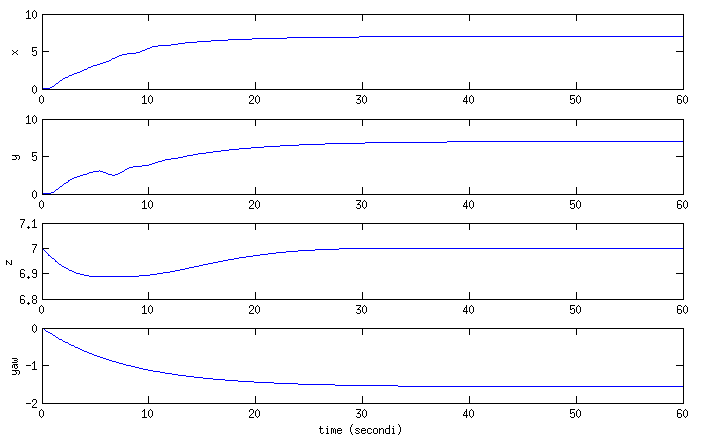
\includegraphics[scale=0.5]{img/plot/matlab/simulation1.png}
\caption{Simulazione n°1, Matlab}
\label{sim:1M}
\end{center}
\end{figure}

\begin{figure}[p]
\hspace*{-3.5cm}
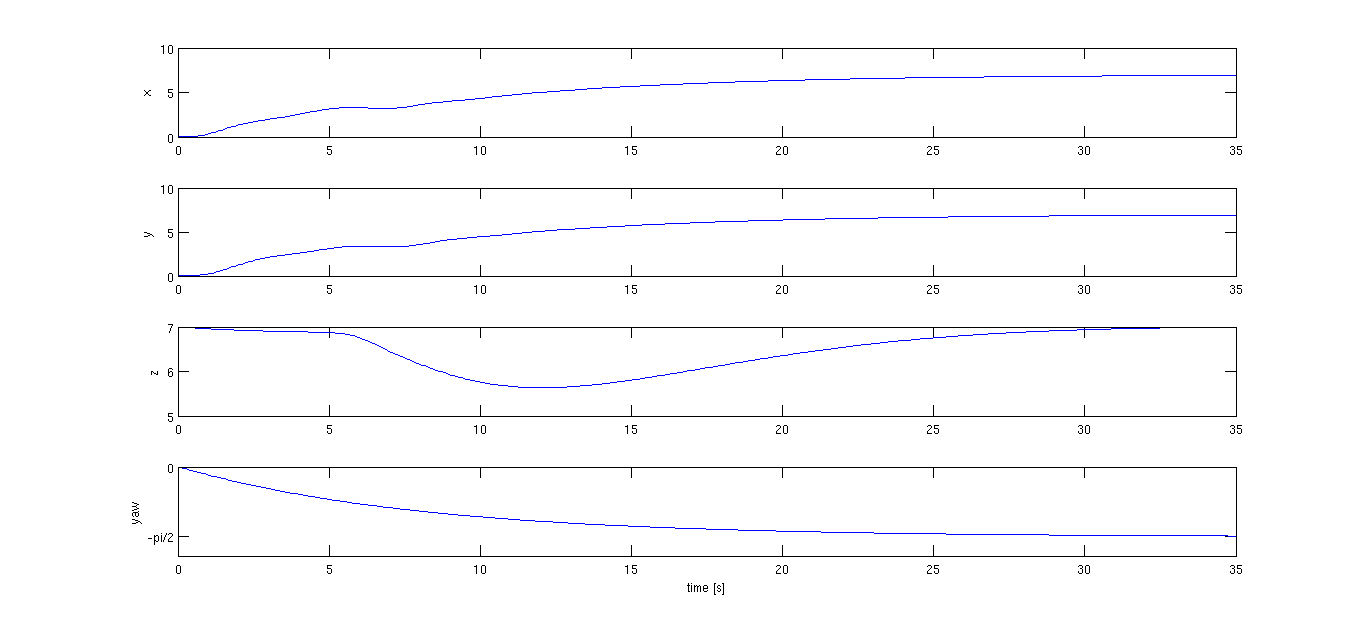
\includegraphics[scale=0.5]{img/plot/matlab/sim2_pdf.png}
\caption{Simulazione n°2, Matlab}
\label{sim:2M}
\end{figure}

\begin{figure}[p]
\hspace*{-3.5cm}
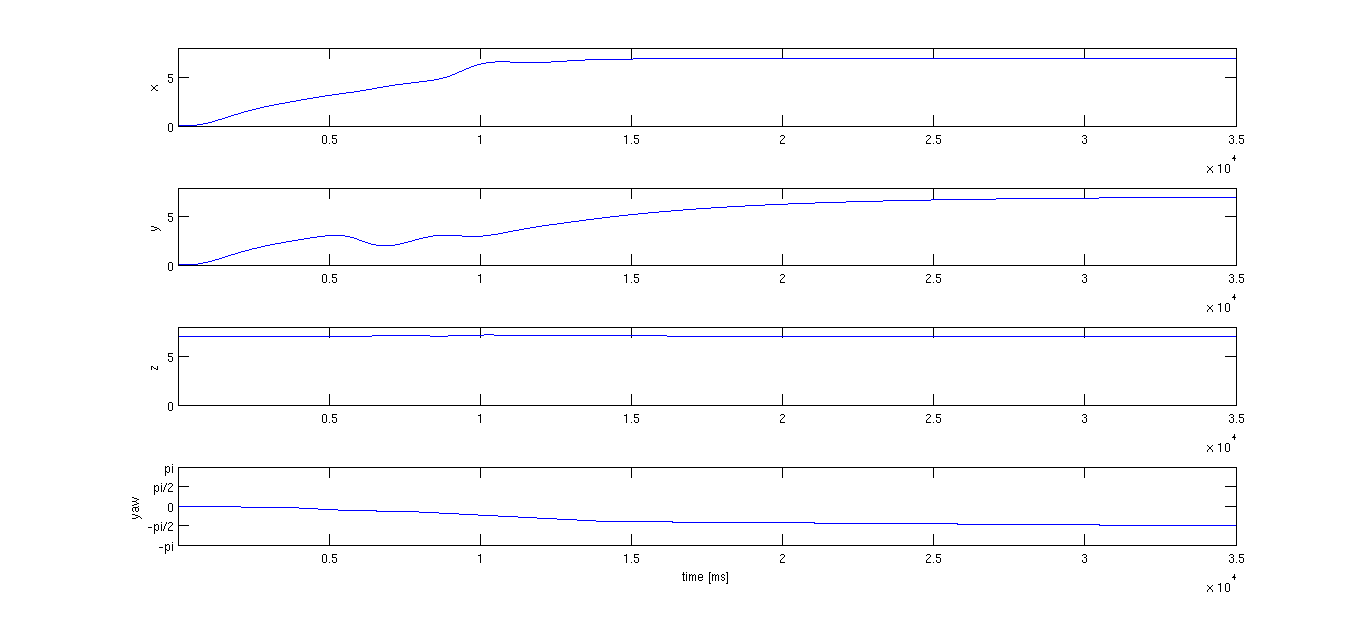
\includegraphics[scale=0.5]{img/plot/gazebo/simulazione1_pdf.png}
\caption{Simulazione n°1, GAZEBO}
\label{sim:1G}
\end{figure}

\begin{figure}[p]
\hspace*{-3.5cm}
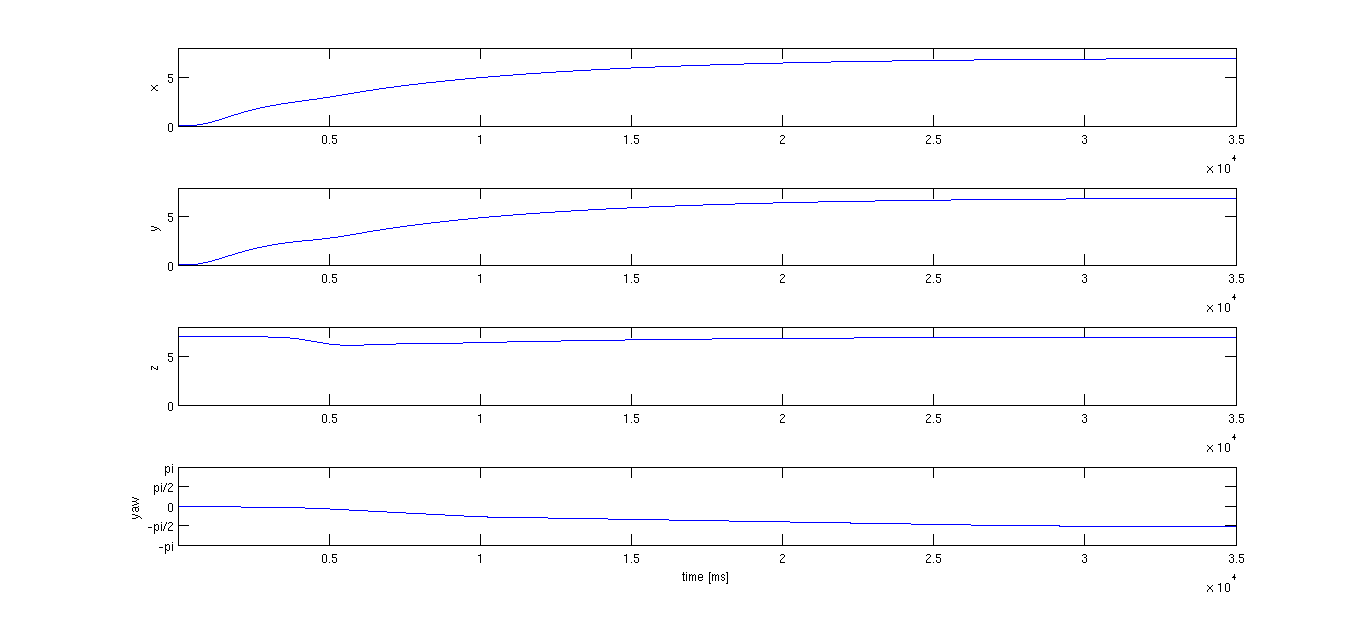
\includegraphics[scale=0.5]{img/plot/gazebo/simulazione2_pdf.png}
\caption{Simulazione n°2, GAZEBO}
\label{sim:2G}
\end{figure}

\begin{figure}[p]
\hspace*{-3.5cm}
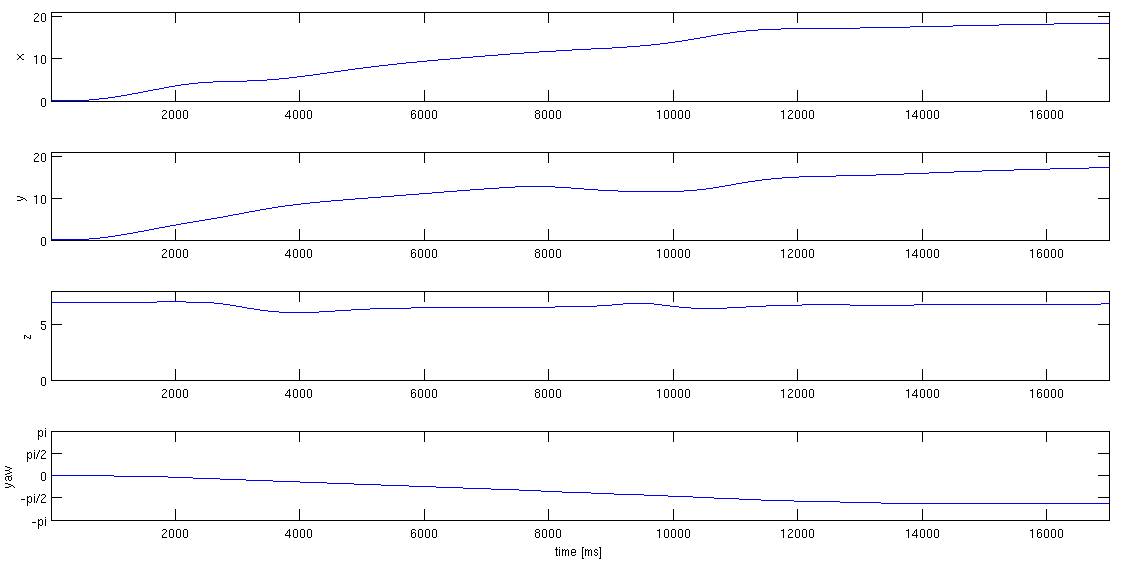
\includegraphics[scale=0.5]{img/plot/gazebo/simulazione3_pdf.png}
\caption{Simulazione n°3, GAZEBO}
\label{sim:3G}
\end{figure}

\FloatBarrier
\newpage

\bibliography{references}
\bibliographystyle{plain}


\end{document}
